\documentclass[12pt]{jsarticle}
\usepackage{geometry}
\geometry{left=10mm,right=15mm,top=15mm,bottom=15mm}
\usepackage{amssymb}
\usepackage{mathcomp}
\usepackage{listings}
\usepackage{amsmath,amsthm} 
\usepackage[dvipdfmx]{graphicx}
\usepackage{txfonts}
\lstset{
  basicstyle={\ttfamily},
  identifierstyle={\small},
  commentstyle={\smallitshape},
  keywordstyle={\small\bfseries},
  ndkeywordstyle={\small},
  stringstyle={\small\ttfamily},
  frame={tb},
  breaklines=true,
  columns=[l]{fullflexible},
  numbers=left,
  xrightmargin=0zw,
  xleftmargin=3zw,
  numberstyle={\scriptsize},
  stepnumber=1,
  numbersep=1zw,
  lineskip=-0.5ex
}
\newenvironment{solution}
  {\renewcommand\qedsymbol{$\blacksquare$}\begin{proof}[Solution]}
  {\end{proof}}
\begin{titlepage}
\title{\Huge{構造振動論 レポート}}
\author{\LARGE{工学部航空宇宙工学科三年 野本陽平 (03-180332)}}
\date{\large{2019年2月5日}}
\thispagestyle{empty}
\end{titlepage}
\begin{document}
\maketitle
\newpage
\section*{はじめに}
数値構造解析のときは, 提出が遅くなったにも関わらず提出を受け入れていただき本当にありがとうございました. それを補うことができるのようなものだとは思っていませんが, 今回は早めに提出させていただきます.
\section*{問題1}
下図に示すような断面が変化するはり(密度$\rho$, ヤング率$E$)の両端自由条件における曲げ振動解析(紙面の面内曲げ振動のみを考える)をこころみる. 一様断面はりの固有振動モードを用い, 断面変化を有するはりの固有振動数および固有モード(図示すること) を3次モードまで求め, 高さ$2h$を有する一様断面はりの場合と比較せよ. ただし, 各断面は幅一定の長方形形状をしており, 必要であれな$\rho=2.7g/cm^3, E=70GPa, h=2mm, l=1000mm$とせよ.
\subsection*{諸物理量の定義}
\begin{solution}
形状が長方形である断面の断面二次モーメントは
\begin{eqnarray*}
I(x)=\cfrac{bh^3}{12}\left(1+\cfrac{2x}{l} \right)
\end{eqnarray*}
よって, 曲げ剛性$EI$と線密度$\mu$は
\begin{eqnarray*}
EI &=& \cfrac{EBh^3}{12}\left(1+\cfrac{2x}{l}\right)^3 \\
\mu &=& \rho bh\left(1+\cfrac{2x}{l}\right)
\end{eqnarray*}
一方で, 高さ$2h$を有する一様断面はりの場合の曲げ剛性$EI_{2h}$と線密度$\mu_{2h}$は,
\begin{eqnarray*}
EI &=& \cfrac{Ebh^3}{12}\times 2^3 = \cfrac{2}{3}Ebh^3 \\
\mu &=& 2\rho bh
\end{eqnarray*}
である. 問題文の順序とは逆行することになるが, 以下では初めに一様断面はりの固有振動を検討し, 次に断面が変化するはりについて考えるものとする.
\subsection*{一様断面はり}
運動方程式
\begin{eqnarray*}
\cfrac{\partial^2}{\partial x^2}\left(EI\cfrac{\partial^2 w}{\partial x^2} \right) + \mu\cfrac{\partial^2 w}{\partial t^2} - \cfrac{\partial}{\partial x}\left(\rho I\cfrac{\partial^3 w}{\partial t^2\partial x} \right) = q_x + \cfrac{\partial m_x}{\partial x}
\end{eqnarray*}
に対して, 外力なし($q_x=0, m_x=0$), 一様断面($EI, \rho I$は$x$の関数ではない), $\rho I \ll EI, \mu$の仮定を代入すると以下のような単純な形にできる.
\begin{eqnarray*}
EI\cfrac{\partial^4 w}{\partial x^4} + \mu\cfrac{\partial^2 w}{\partial t^2} = 0
\end{eqnarray*}
理論解を$w(x,t)=u(x)v(t)$なる変数分離でおき, 近似されたEOMに代入すると,
\begin{eqnarray*}
EIu(t)\cfrac{d^4 u(x)}{d x^4} + \mu u(x)\cfrac{d^2 v(t)}{dt^2} &=& 0
\quad \Rightarrow \quad \cfrac{\frac{d^2 v}{dt^2}}{v} = -\cfrac{EI\frac{d^4 u}{dx^4}}{\mu u} \equiv -\omega^2 \\
\therefore \cfrac{d^2 v}{dt^2} + \omega^2 v &=& 0, \quad \cfrac{d^4 u}{dx^4} - \left(\cfrac{\lambda}{l} \right)^4 u = 0
\end{eqnarray*}
ただし解析的に計算しやすくするために$\lambda^4 \equiv \frac{\mu \omega^2 l^4}{EI}$とおいている. それぞれを解くと,
\begin{eqnarray*}
u(x) &=& A\cos\omega t + B\sin\omega t \\
v(t) &=& C_1\cosh\cfrac{\lambda x}{l} + C_2\cos\cfrac{\lambda x}{l} + C_3\sinh\cfrac{\lambda x}{l} + C_4\sin\cfrac{\lambda x}{l}
\end{eqnarray*}
である. 両端が自由端であるから, 剪断力及び曲げモーメントから境界条件$x=0, l: \frac{d^2 u}{dx^2} = \frac{d^3 u}{dx^3} = 0$を得る. これを代入・整理して行列形式にすると,
\begin{eqnarray*}
\left[
\begin{array}{cccc}
(\frac{\lambda}{l})^2 & -(\frac{\lambda}{l})^2 & 0 & 0 \\
0 & 0 & (\frac{\lambda}{l})^2 & -(\frac{\lambda}{l})^2 \\
(\frac{\lambda}{l})^2\cosh\lambda & -(\frac{\lambda}{l})^2\cos\lambda & (\frac{\lambda}{l})^2\sinh\lambda & -(\frac{\lambda}{l})^2\sin\lambda \\
(\frac{\lambda}{l})^3\sinh\lambda & (\frac{\lambda}{l})^3\sin\lambda & (\frac{\lambda}{l})^3\cosh\lambda & -(\frac{\lambda}{l})^3\cos\lambda \\
\end{array}
\right]
\left[
\begin{array}{c}
C_1 \\ C_2 \\ C_3 \\ C_4 \\
\end{array}
\right]
= \left[
\begin{array}{c}
0 \\ 0 \\ 0 \\ 0 \\
\end{array}
\right]
\end{eqnarray*}
上の行列が非自明解を持つのは行列の行列式が0になる時であり, 上の行列を$A$とおくと
\begin{eqnarray*}
\det A = 0 \Leftrightarrow \cosh\lambda\cos\lambda -1=0
\end{eqnarray*}
これらの条件を加味すると, $\left[
\begin{array}{cccc}
C_1 & C_2 & C_3 & C_4
\end{array}
\right]^T$は以下のように表される.
\begin{eqnarray*}
\left[
\begin{array}{c}
C_1 \\ C_2 \\ C_3 \\ C_4 \\
\end{array}
\right]
=\left[
\begin{array}{c}
1 \\ 1 \\ -\frac{\sinh\lambda+\sin\lambda}{\cosh\lambda-\cos\lambda} \\ -\frac{\sinh\lambda+\sin\lambda}{\cosh\lambda-\cos\lambda} \\
\end{array}
\right]C_1
\end{eqnarray*}
この$C_1$は振幅を表すファクターなので, 固有振動の固有振動数を考える際には適当に決めて良い. 故にここでは1とする. よって$u(x)$は
\begin{eqnarray*}
u_r(x) = \cosh\cfrac{\lambda_r x}{l} + \cos\cfrac{\lambda_r x}{l} -\beta\left(\sinh\cfrac{\lambda_r x}{l} + \sin\cfrac{\lambda_r x}{l} \right)
\end{eqnarray*}
となる. ただし$\lambda_r$は$\cosh\lambda\cos\lambda-1=0$の解を小さい順(=低次の振動モードを示す順)に並べたものを$\lambda_1, \lambda_2, ...$と定義したものであり, 各$\lambda_r$は[2]より数値計算で求めるものとする. なお, これらの値はシステム学実験で扱ったReference[1]の情報とも概ね一致しているから正しいものと判断できる; 今回はwolframで求めた. wolframについてはReference[2]を参照.
\begin{eqnarray*}
\left\{
\begin{array}{l} 
\lambda_1 \approx 4.7300407448627 \\
\lambda_2 \approx 7.8532046240958 \\
\lambda_3 \approx 10.995607838002\\
\lambda_4 \approx 14.137165491258 \\
\end{array}
\right.
\end{eqnarray*}
一方, $\omega_r = (\frac{\lambda_r}{l})^2\sqrt{\frac{EI}{\mu}} = (\frac{\lambda_r}{l})^2\sqrt{\frac{Eh^2}{3\rho}}$であるから, 固有角振動数$\omega_r$は
\begin{eqnarray*}
\left\{
\begin{array}{l} 
\omega_1 \approx 131.54255401562 \quad [rad/s] \\
\omega_2 \approx 362.60211546633 \quad [rad/s] \\
\omega_3 \approx 710.84512705380 \quad [rad/s] \\
\omega_4 \approx 1175.0631042471 \quad [rad/s] \\
\end{array}
\right.
\end{eqnarray*}
\subsection*{テーパー梁}
Rayleigh-Ritz法を用いて解く. はりの振動波形$W(x)$は変異境界条件を満たす関数$\phi_i(x)$を用いて
\begin{eqnarray*}
W^*(x)=\Sigma_{i=1}^4C_i\phi_i(x)
\end{eqnarray*}
によって表すことができる. ただし,
\begin{eqnarray*}
\phi_i = \cosh\cfrac{\lambda_i x}{l} + \cos\cfrac{\lambda_i x}{l} -\beta\left(\sinh\cfrac{\lambda_i x}{l} + \sin\cfrac{\lambda_i x}{l} \right)
\end{eqnarray*}
とする. 質量マトリックス$M^{\ast}$, 剛性マトリックス$K^{\ast}$
\begin{eqnarray*}
M^{\ast} &=& \int_0^l \mu \left[
\begin{array}{c}
\phi_1 \\ \phi_2 \\ \phi_3 \\ \phi_4 \\
\end{array}
\right]\left[
\begin{array}{cccc}
\phi_1 & \phi_2 & \phi_3 & \phi_4 \\
\end{array}
\right]dx =
\int_0^l \rho h\left(1+\cfrac{2x}{l}\right) \left[
\begin{array}{c}
\phi_1 \\ \phi_2 \\ \phi_3 \\ \phi_4 \\
\end{array}
\right]\left[
\begin{array}{cccc}
\phi_1 & \phi_2 & \phi_3 & \phi_4 \\
\end{array}
\right]dx \\
K^{\ast} &=& \int_0^l EI \left[
\begin{array}{c}
\phi_1 \\ \phi_2 \\ \phi_3 \\ \phi_4 \\
\end{array}
\right]\left[
\begin{array}{cccc}
\phi_1 & \phi_2 & \phi_3 & \phi_4 \\
\end{array}
\right]dx =
\int_0^l \cfrac{Eh^3}{12}\left(1+\cfrac{2x}{l}\right)^3 \left[
\begin{array}{c}
\phi_1 \\ \phi_2 \\ \phi_3 \\ \phi_4 \\
\end{array}
\right]\left[
\begin{array}{cccc}
\phi_1 & \phi_2 & \phi_3 & \phi_4 \\
\end{array}
\right]dx
\end{eqnarray*}
より, $M^{\ast-1}$を左からかける変形を用いて,
\begin{eqnarray*}
\left[
\begin{array}{c}
K^{\ast} - \omega^2M^{\ast} \\
\end{array}
\right]\left[
\begin{array}{c}
C_1 \\ C_2 \\ C_3 \\ C_4 \\
\end{array}
\right] = 0 \quad\Leftrightarrow\quad \left[
\begin{array}{c}
M^{\ast-1}K^{\ast} - \omega^2I \\
\end{array}
\right]\left[
\begin{array}{c}
C_1 \\ C_2 \\ C_3 \\ C_4 \\
\end{array}
\right]=0
\end{eqnarray*}
これが非自明解を持つ条件は,
\begin{eqnarray*}
det(M^{\ast-1}K^{\ast} - \omega^2I) = 0
\end{eqnarray*}
である. したがって$\omega$は$M^{\ast-1}K^{\ast}$の固有値として, 各モードに対応する$\left[
\begin{array}{cccc}
C_1 & C_2 & C_3 & C_4 \\
\end{array}
\right]^T$が$M^{\ast-1}K^{\ast}$の固有ベクトルとして求めることができる. 今回これを台形近似による数値計算で求めると, モード1からモード4までの比較グラフとテーブルは図1, 2, 3, 4, 5, 6と表1のようになった. なお, テーパー梁のコードはAppendixのtrapezoid.pyを参照. \newline
質量マトリックスの要素が厚みに比例するのに対し, 剛性マトリックスの要素は厚みの3乗に比例するためテーパー梁は全体として剛になる(=固有角振動数が大きくなる)ことが予想されるが, 今回はそのような結果が得られていない. 果たしてこの結果は妥当なのだろうか. $x$方向の分割数$N$を大きくしてもいいのだが, それでは芸がなくpythonを使っている今回は計算時間もかなり長くなってしまうため, シンプソン法を用いる. シンプソン法に関する理論はReference[3]を参照. モード1からモード4までの比較グラフとテーブルは図7, 8, 9, 10, 11, 12と表2のようになった. これより確かに全ての固有角振動数において一様梁の理論解を上回っている. 具体的に用いたコードについてはAppendixのSimpson.pyを参照. 冗長になってしまうためコードは一部のみの抜粋としたが, この関数をtrapezoid.pyの同じ名前の関数と入れ替えれば実行できる.
\end{solution}
\begin{table}[htb]
  \begin{center}
    \caption{テーパー梁の固有角振動数と固有ベクトル(台形近似)}
    \begin{tabular}{|c|cccc|} \hline
       & モード1 & モード2 & モード3 & モード4  \\ \hline
      $\omega$[rad/s] & 125.77 & 350.61 & 695.62 & 1303.06 \\ \hline
      $C_1$ & -0.9962 & -0.1570 & 0.1648 & 0.0024 \\ \hline      
      $C_2$ & 0.0819 & 0.9856 & -0.2809 & -0.0353 \\ \hline
      $C_3$ & 0.0073 & 0.0615 & 0.9530 & 0.3054 \\ \hline
      $C_4$ & 0.0284 & -0.0084 & 0.1123 & -0.9516 \\ \hline
    \end{tabular}
  \end{center}
\end{table}
\begin{table}[htb]
  \begin{center}
    \caption{テーパー梁の固有角振動数と固有ベクトル(シンプソン近似)}
    \begin{tabular}{|c|cccc|} \hline
       & モード1 & モード2 & モード3 & モード4  \\ \hline
      $\omega$[rad/s] & 154.04 & 429.40 & 851.95 & 1595.92 \\ \hline
      $C_1$ & -0.9962 & -0.1570 & 0.1648 & 0.0024 \\ \hline      
      $C_2$ & 0.0819 & 0.9856 & -0.2809 & -0.0353 \\ \hline
      $C_3$ & 0.0073 & 0.0615 & 0.9530 & 0.3054 \\ \hline
      $C_4$ & 0.0284 & -0.0084 & 0.1123 & -0.9516 \\ \hline
    \end{tabular}
  \end{center}
\end{table} 
\newpage
\begin{figure}[htbp]
 \begin{minipage}{0.5\hsize}
  \begin{center}
   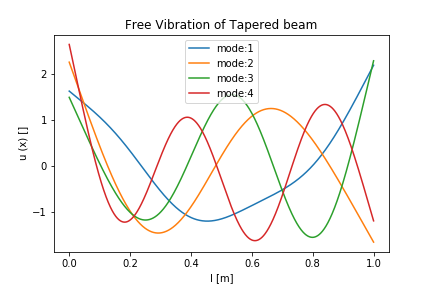
\includegraphics[width=70mm]{fig1.png}
   \caption{}
  \end{center}
  \label{fig:one}
 \end{minipage}
 \begin{minipage}{0.5\hsize}
  \begin{center}
   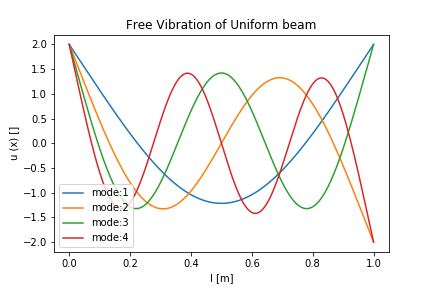
\includegraphics[width=70mm]{fig2.png}
   \caption{}   
  \end{center}
  \label{fig:two}
 \end{minipage}
\end{figure}
\begin{figure}[htbp]
 \begin{minipage}{0.5\hsize}
  \begin{center}
   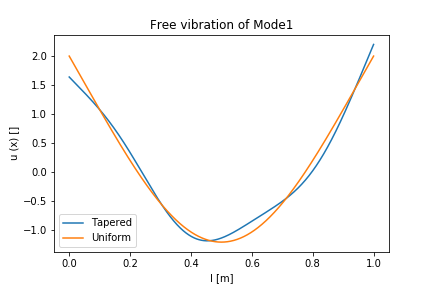
\includegraphics[width=70mm]{fig3.png}
   \caption{}   
  \end{center}
  \label{fig:one}
 \end{minipage}
 \begin{minipage}{0.5\hsize}
  \begin{center}
   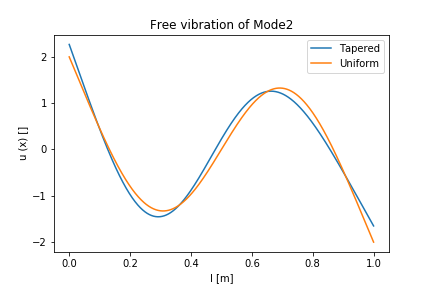
\includegraphics[width=70mm]{fig4.png}
   \caption{}   
  \end{center}
  \label{fig:two}
 \end{minipage}
\end{figure}
\begin{figure}[htbp]
 \begin{minipage}{0.5\hsize}
  \begin{center}
   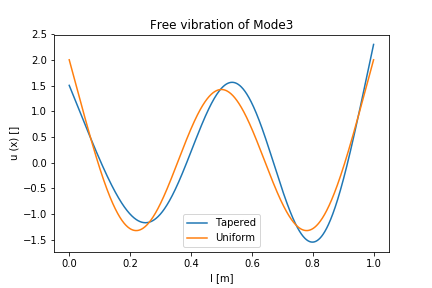
\includegraphics[width=70mm]{fig5.png}
   \caption{}   
  \end{center}
  \label{fig:one}
 \end{minipage}
 \begin{minipage}{0.5\hsize}
  \begin{center}
   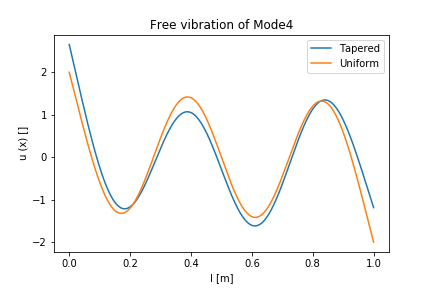
\includegraphics[width=70mm]{fig6.png}
   \caption{}   
  \end{center}
  \label{fig:two}
 \end{minipage}
\end{figure}
\begin{figure}[htbp]
 \begin{minipage}{0.5\hsize}
  \begin{center}
   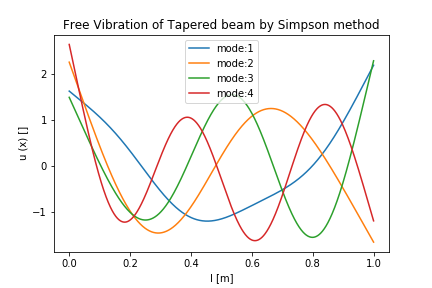
\includegraphics[width=70mm]{fig7.png}
   \caption{}   
  \end{center}
  \label{fig:one}
 \end{minipage}
 \begin{minipage}{0.5\hsize}
  \begin{center}
   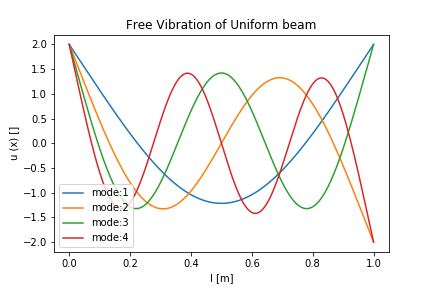
\includegraphics[width=70mm]{fig8.png}
   \caption{}   
  \end{center}
  \label{fig:two}
 \end{minipage}
\end{figure}
\begin{figure}[htbp]
 \begin{minipage}{0.5\hsize}
  \begin{center}
   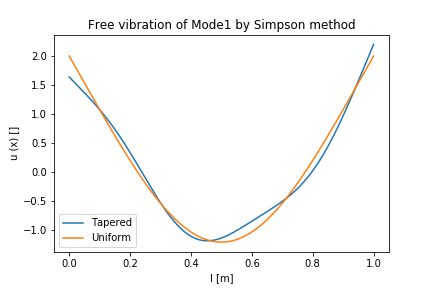
\includegraphics[width=70mm]{fig9.png}
   \caption{}   
  \end{center}
  \label{fig:one}
 \end{minipage}
 \begin{minipage}{0.5\hsize}
  \begin{center}
   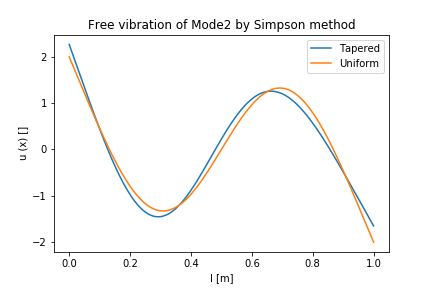
\includegraphics[width=70mm]{fig10.png}
   \caption{}   
  \end{center}
  \label{fig:two}
 \end{minipage}
\end{figure}
\begin{figure}[htbp]
 \begin{minipage}{0.5\hsize}
  \begin{center}
   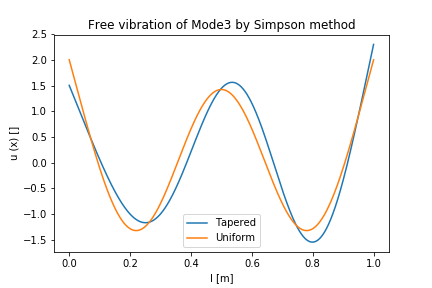
\includegraphics[width=70mm]{fig11.png}
   \caption{}   
  \end{center}
  \label{fig:one}
 \end{minipage}
 \begin{minipage}{0.5\hsize}
  \begin{center}
   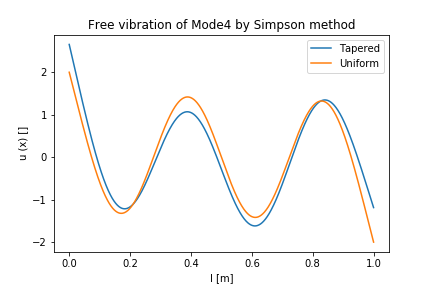
\includegraphics[width=70mm]{fig12.png}
   \caption{}   
  \end{center}
  \label{fig:two}
 \end{minipage}
\end{figure}
\newpage
\section*{問題2}
下図に示すように, 質量$m$の剛体が速さ$V_0$で棒(密度$\rho$, ヤング率$E$, 断面積$A$)に衝突したとする. このとき, 以下の問いに答えよ. 尚, 棒の左端を原点とする$x$座標を図のように定める.
\begin{enumerate}
\item 棒を$x$の正方向に伝える縦波$u=f(\xi )=f(x-at)$を考える($a$は位相速度). 棒に発生する応力と速度の関係を$\rho, a$を用いて表せ.
\begin{solution}
$u=f(\xi)$をxとtで偏微分する.
\begin{eqnarray*}
\cfrac{\partial u}{\partial x} &=& \cfrac{\partial \xi}{\partial x}\cfrac{\partial f}{\partial \xi} = \cfrac{\partial(x-at)}{\partial x}\cfrac{\partial f}{\partial \xi} = \cfrac{\partial f}{\partial \xi} \\
\cfrac{\partial u}{\partial t} &=& \cfrac{\partial \xi}{\partial t}\cfrac{\partial f}{\partial \xi} = \cfrac{\partial(x-at)}{\partial t}\cfrac{\partial f}{\partial \xi} = -a\cfrac{\partial f}{\partial \xi}
\end{eqnarray*}
棒に発生する応力を$\sigma(x, t)$と表すと,
\begin{eqnarray*}
\sigma(x,t) = E\cfrac{\partial u}{\partial x} = E\cfrac{\partial f}{\partial \xi} = -\cfrac{E}{a}\cfrac{\partial u}{\partial t} = \underline{-\rho a\cfrac{\partial u}{\partial t}}
\end{eqnarray*}
但し最後の変形では位相速度$a$についての式$a^2=\frac{E}{\rho}$を用いた.
\end{solution}
\item 剛体と棒が接触している際, 剛体と左端面は同じ速度を持つと考えられる. このとき, 棒左端($x=0$)の応力$\sigma_0(t)$と剛体速度$V(t)$の関係を示せ. また, 棒からの反力を考え, 接触している間の剛体の運動方程式を示せ.
\begin{solution}
剛体と棒が接触しているとき, 剛体と左端面は同じ速度を持つ. 故に剛体速度$V(t)$を用いると
\begin{eqnarray*}
\sigma_0(t) = \sigma(0,t) = -\rho a \left.\cfrac{\partial u}{\partial t}\right |_{x=0} = -\rho a V(t)
\end{eqnarray*}
応力は引張が正であるから,
\begin{eqnarray*}
m\cfrac{dV}{dt} = \sigma_0(t)A = \underline{-\rho aAV(t)}
\end{eqnarray*}
\end{solution}
\item (2)の2式から, 棒左端の応力$\sigma_0(t)$の満たすべき微分方程式を求め, $\sigma_0(t)$を求めよ. ただし, 衝突時を$t=0$とし, そのとき, 棒左端の速度は$V_0$と等しいと考えてよい.
\begin{solution}
$V(t)$の式を剛体の運動方程式に代入すると,
\begin{eqnarray*}
\cfrac{d}{dt}\sigma_0(t) = -\cfrac{\rho aA}{m}\sigma_0(t)
\end{eqnarray*}
これを解くことで, 不定積分込みの$\sigma_0(t)$を得る.
\begin{eqnarray*}
\sigma_0(t) = C\exp\left(-\cfrac{\rho aA}{m} t \right)
\end{eqnarray*}
初期条件$V(0)=V_0 \Rightarrow \sigma_0(0) = C = -\rho aV_0$を代入して完全な$\sigma_0(t)$を得る.
\begin{eqnarray*}
\sigma_0(t)=\underline{-\rho aV_0\exp\left(-\cfrac{\rho aA}{m}t \right)}
\end{eqnarray*}
\end{solution}
\item 縦波の運動方程式を棒内部の応力を用いて表し, $x$の正方向に伝わる応力波$\sigma(x, t)=g(x-at)$はこの運動方程式の解であることを示せ.
\begin{proof}
今外力なしで一様断面の物体に対する縦波の運動方程式を考える. これを整理すると,
\begin{eqnarray*}
\cfrac{\partial}{\partial}\left(EA\cfrac{\partial u}{\partial x} \right) + P_x = \rho A \cfrac{\partial^2 u}{\partial t^2} \\
\Rightarrow \quad EA\cfrac{\partial^2 u}{\partial x^2} = \rho A\cfrac{\partial^2 u}{\partial t^2} \\
\Rightarrow \quad \cfrac{\partial^2 u}{\partial t^2}=a^2\cfrac{\partial^2 u}{\partial x^2}
\end{eqnarray*}
また, $E$が定数であることから,
\begin{eqnarray*}
\sigma(x,t) &=& E\cfrac{\partial u}{\partial x}
\Rightarrow \cfrac{\partial \sigma}{\partial x} = E\cfrac{\partial^2 u}{\partial x^2} \\
\therefore \cfrac{\partial \sigma}{\partial x} &=& \rho \cfrac{\partial^2 u}{\partial t^2}
\end{eqnarray*}
両辺を$x$で偏微分し, 偏微分を交代させると棒内部の応力による縦波の運動方程式を得る.
\begin{eqnarray*}
\cfrac{\partial^2 \sigma}{\partial x^2} &=& \rho \cfrac{\partial}{\partial x}\left(\cfrac{\partial^2 u}{\partial t^2} \right) = \rho \cfrac{\partial^2}{\partial t^2}\left(\cfrac{\partial u}{\partial x} \right) = \cfrac{\rho}{E} \cfrac{\partial^2 \sigma}{\partial t^2} \\
\therefore \cfrac{\partial^2 \sigma}{\partial^2 t} &=& \cfrac{E}{\rho}\cfrac{\partial^2 \sigma}{\partial x^2} = a^2\cfrac{\partial^2 \sigma}{\partial x^2}
\end{eqnarray*}
これに対し$\sigma(x, t)=g(x-at)$を代入し, 運動方程式の解であることを示すことができる.
\begin{eqnarray*}
\cfrac{\partial^2 \sigma}{\partial t^2} &=& \cfrac{\partial(x-at)}{\partial t}\cfrac{\partial}{\partial(x-at)}\left(\cfrac{\partial \sigma}{\partial t}\right) = -a\cfrac{\partial}{\partial(x-at)}\left(\cfrac{\partial (x-at)}{\partial t}\cfrac{\partial g}{\partial (x-at)}\right) = a^2\cfrac{\partial^2 g}{\partial (x-at)^2} \\
\cfrac{\partial^2 \sigma}{\partial x^2} &=&\cfrac{\partial(x-at)}{\partial x}\cfrac{\partial}{\partial(x-at)}\left(\cfrac{\partial \sigma}{\partial x}\right) = \cfrac{\partial}{\partial(x-at)}\left(\cfrac{\partial (x-at)}{\partial x}\cfrac{\partial g}{\partial (x-at)}\right) = \cfrac{\partial^2 g}{\partial (x-at)^2}
\end{eqnarray*}
以上より, 確かに運動方程式の解として正しい.
\end{proof}
\item 棒内部へはどのような縦波(応力波)が伝搬するか. 衝突から$t$秒後の棒内部の応力状態を図示せよ.
\begin{solution}
3, 4で得た結論によると,
\begin{eqnarray*}
\sigma_0(t)=-\rho aV_0\exp\left(-\cfrac{\rho aA}{m}t \right) = g(-at)
\end{eqnarray*}
$g$は$x-at$による関数であることを踏まえると, 伝播を表す$g$と衝突を表す$\sigma_0$の間に以下のような関係があると考えて矛盾はない.
\begin{eqnarray*}
\underline{g(x-at) = -\rho a V_0\exp\left(\cfrac{\rho A}{m}(x-at) \right)}
\end{eqnarray*}
これを図示すると以下のようになる. ただし, \underline{$at<x$には衝撃が伝播していないため, 応力が存在しない.}
\end{solution}
\end{enumerate}
\newpage
\section*{Appendix}
\begin{lstlisting}[caption=trapezoid.py,label=fuga]
#!/usr/bin/env python3
# -*- coding: utf-8 -*-
"""
Created on Sun Jan 27 05:24:06 2019

@author: yohei
"""

import numpy as np
import matplotlib.pyplot as plt

E = 70 * (10 ** 9) #youngs_modulus[Pa]
h = 0.002 #thickness[m]
rho = 2700 #desity[kg/m^3]
l = 1 #length[m]
lambda_r = np.array([4.7300407448627,
                     7.8532046240958,
                     10.995607838002,
                     14.137165491258])
beta = np.zeros(4)
for i in range(len(beta)):
    beta[i] += (np.cosh(lambda_r[i])-np.cos(lambda_r[i]))/(np.sinh(lambda_r[i])-np.sin(lambda_r[i]))
        
class BEF: #Both Edge Free  
    def __init__(self):
        self.N = 1000 #division number
        self.x_ = np.linspace(0, l, self.N)
    
    def phi(self, x):
        phi = np.array([np.cosh(lambda_r[i]*x/l) + np.cos(lambda_r[i]*x/l) - beta[i]*(np.sinh(lambda_r[i]*x/l)+np.sin(lambda_r[i]*x/l)) for i in range(4)])
        dif = np.array([(lambda_r[i]/l)**2 for i in range(4)])
        ddphi = np.array([dif[i]*(np.cosh(lambda_r[i]*x/l) - np.cos(lambda_r[i]*x/l) - beta[i]*(np.sinh(lambda_r[i]*x/l)-np.sin(lambda_r[i]*x/l))) for i in range(4)])
        return phi, ddphi
     
    def f(self, x):
        EI = E * h**3 * (1 + 2*x/l)**3 / 12
        phi_for_EI = [[],[],[],[]]
        ddphi = self.phi(x)[1]
        for i in range(4):
            for j in range(4):
                phi_for_EI[i].append(ddphi[i]*ddphi[j]*EI)
        return phi_for_EI
    
    def g(self, x):
        mu = rho*h*(1+2*x/l)
        phi_for_mu = [[],[],[],[]]
        phi = self.phi(x)[0]
        for i in range(4):
            for j in range(4):
                phi_for_mu[i].append(phi[i]*phi[j]*mu)
        return phi_for_mu
    
    def K(self):
        K = np.zeros((4,4))
        for i in range(4):
            for j in range(4):
                for k in range(len(self.x_)-1):
                    y=(self.f(self.x_[k])[i][j]+self.f(self.x_[k+1])[i][j])/2
                    K[i][j]+=(self.x_[k+1]-self.x_[k])*y
        return K
    
    def M(self):
        M = np.zeros((4,4))
        for i in range(0,4):
            for j in range(0,4):
                for k in range(len(self.x_)-1):
                    y=(self.g(self.x_[k])[i][j]+self.g(self.x_[k+1])[i][j])/2
                    M[i][j]+=(self.x_[k+1]-self.x_[k])*y 
        return M
    
    def eigen(self):
        M_inv = np.linalg.inv(self.M())
        dots = np.dot(M_inv, self.K())
        eigenvalue, eigenvector = np.linalg.eig(dots.T)
        return np.sqrt(eigenvalue), eigenvector

    def discretization(self):
        ector = self.eigen()[1]
        y = np.zeros((4,len(self.x_)))
        for k in range(4):
            for i in range(len(self.x_)):
                temp = 0
                n = self.x_[i]
                for j in range(4):
                    temp += ector[k][j]*self.phi(n)[0][j]
                y[k][i] = temp
        return y        

    def describe_tapered(self):
        y = self.discretization()
        plt.title("Free Vibration of Tapered beam")
        plt.plot(self.x_, -y[3], label="mode:1")
        plt.plot(self.x_, -y[0], label="mode:2")
        plt.plot(self.x_, y[1], label="mode:3")
        plt.plot(self.x_, y[2], label="mode:4")
        plt.legend()
        plt.xlabel("l [m]")
        plt.ylabel("u (x) []")
        plt.savefig('fig1.png')
        
    def describe_uniform(self):
        y = self.phi(self.x_)
        plt.title("Free Vibration of Uniform beam")
        for i in range(4):
            plt.plot(self.x_, y[0][i], label="mode:"+ str(i+1))
        plt.legend()
        plt.xlabel("l [m]")
        plt.ylabel("u (x) []")
        plt.savefig('fig2.png')
    
    def describe_mode1(self):
        y1 = self.discretization()
        y2 = self.phi(self.x_)
        plt.title("Free vibration of Mode1")
        plt.plot(self.x_, -y1[3], label="Tapered")
        plt.plot(self.x_, y2[0][0], label="Uniform")
        plt.legend()
        plt.xlabel("l [m]")
        plt.ylabel("u (x) []")
        plt.savefig('fig3.png')
        
    def describe_mode2(self):
        y1 = self.discretization()
        y2 = self.phi(self.x_)
        plt.title("Free vibration of Mode2")
        plt.plot(self.x_, -y1[0], label="Tapered")
        plt.plot(self.x_, y2[0][1], label="Uniform")
        plt.legend()
        plt.xlabel("l [m]")
        plt.ylabel("u (x) []")
        plt.savefig('fig4.png')
        
    def describe_mode3(self):
        y1 = self.discretization()
        y2 = self.phi(self.x_)
        plt.title("Free vibration of Mode3")
        plt.plot(self.x_, y1[1], label="Tapered")
        plt.plot(self.x_, y2[0][2], label="Uniform")
        plt.legend()
        plt.xlabel("l [m]")
        plt.ylabel("u (x) []")
        plt.savefig('fig5.png')
        
    def describe_mode4(self):
        y1 = self.discretization()
        y2 = self.phi(self.x_)
        plt.title("Free vibration of Mode4")
        plt.plot(self.x_, y1[2], label="Tapered")
        plt.plot(self.x_, y2[0][3], label="Uniform")
        plt.legend()
        plt.xlabel("l [m]")
        plt.ylabel("u (x) []")
        plt.savefig('fig6.png')

def free_vibration():
    root = np.sqrt((E*(h**2))/(3*rho))
    temp = []
    for i in range(len(lambda_r)):
        temp.append(root*(lambda_r[i]**2)/l**2)
    return temp

if __name__ == '__main__':
    bef = BEF()
    #uni = uniform()
    print("Eigenvalue and Eigenvector", bef.eigen())
    print("equivalent to Eigenvalue of free vibration", free_vibration())
    #bef.describe_tapered()
    #bef.describe_uniform()
    #bef.describe_mode1()
    #bef.describe_mode2()
    #bef.describe_mode3()
    bef.describe_mode4()
\end{lstlisting}
\begin{lstlisting}[caption=Simpson.py,label=fuga]
    def discretization(self):
        ector = self.eigen()[1]
        y = np.zeros((4,len(self.x_)))
        for k in range(4):
            for i in range(len(self.x_)):
                temp = 0
                n = self.x_[i]
                for j in range(4):
                    temp += ector[k][j]*self.phi(n)[0][j]
                y[k][i] = temp
        return y        
\end{lstlisting}
\section*{Reference} \noindent
[1] "Vibration of Redtangular Plates by the Ritz Method" by DANA YOUNG \newline
[2] https://www.wolframalpha.com \newline
[3] https://qiita.com/popondeli/items/fbc602b80223227f3d0e
\end{document}